\title{\textbf{Segmentación de Tumores Cerebrales en Imágenes por Resonancia Magnética}}
\author{\small Máximo D. Utrera, Facultad de Ingeniería, UBA, Buenos Aires, Argentina \hfill \small \today}
\date{}

\twocolumn[
\begin{@twocolumnfalse}
  \maketitle
  \thispagestyle{fancy}
\end{@twocolumnfalse}
]

\section*{Resumen}

En este trabajo se explora la aplicación de técnicas de aprendizaje profundo para la segmentación semántica de tumores cerebrales a partir de volúmenes de Resonancia Magnética (RMI) en 3D. El problema abordado toma inspiración del desafío BraTS (Brain Tumor Segmentation) y se basa en el procesamiento de 4 canales de imagen (T1, T1CE, T2, FLAIR). Se propone una solución que incluye el preprocesamiento robusto de los datos, descartando volúmenes con poca anotación, normalizando el espacio de vóxeles (pixeles volumétricos) y recortando las imágenes a 128x128x128. Inicialmente se consideró el uso de modelos eficientes de bajos recursos, por lo que se experimentó con arquitecturas como MobileNetV2 acoplado a U-Net. Sin embargo, para procesar la totalidad del dataset tridimensional (+40GB), se consolidó un modelo 3D U-Net estándar. Los resultados obtenidos evidencian la viabilidad de la arquitectura, logrando un Dice Score promedio de 0.73 y un IoU de 0.61 en validación a través de múltiples clases (NCR, ED, ET). En etapas futuras se busca aportar también explicabilidad e incertidumbre para mayor confiabilidad clínica.
\vspace{0.25cm}

\section{Introducción}

La segmentación automática de tumores cerebrales representa un avance tecnológico trascendental en el ámbito médico, permitiendo asistir a neuro-radiólogos en el análisis y diagnóstico utilizando Resonancias Magnéticas. En la distribución proporcionada por el desafío BraTS, cada caso clínico contiene inicialmente 4 volúmenes para representar diferentes contrastes: T1, T1CE, T2 y FLAIR.

Las etiquetas de los tejidos proporcionados consisten en regiones de fondo no útiles, tejido necrótico y 'non-enhancing tumor' (NCR/NET), edema (ED) y 'enhancing tumor' ET).

Este proyecto nace de la motivación por resolver el problema haciendo uso de técnicas de visión por computadora y ahondar en la arquitectura de redes neuronales profundas capaces de lograr una buena inferencia de las etiquetas mencionadas.
Adicionalmente se abordara la evaluación que se hizo respecto a la portabilidad de los modelos y las conclusiones que se tomaron al respecto para finalmente optar por una red U-net mas tradicional, así como también se mencionan posibles mejoras.

\section{Búsqueda del Dataset e Investigación}

Se comenzó el proyecto partiendo de una base de investigación y relevamiento de una variedad de \textit{papers} que abordan el tema o temas allegados tanto desde un punto de vista medico como de redes neuronales (los mismos se pueden encontrar en la sección de referencias).

Luego se llevo a cabo la elección de un dataset que cumpla con el problema a resolver y tenga una cantidad de datos para entrenamiento razonable y que los mismos sean utilizables.

\subsection{Selección de datos}

Para esta etapa se realizó la búsqueda (a través de Kaggle) de distintos conjuntos de datos, el importe de cada uno de ellos y un análisis exploratorio de los mismos que se podrán encontrar en la sección \textbf{notebooks/} dentro del código del proyecto en formato \textit{jupyter notebook}. Luego del análisis llevado a cabo, se decidió descartar los datos menos compatibles con el foco del proyecto y se tomo uno como fijo.

A continuación se listan los conjuntos de datos evaluados y las razones por las que se descartaron:

\vspace{0.5cm}

\begin{itemize}
    \item \textbf{\href{https://www.kaggle.com/datasets/navoneel/brain-mri-images-for-brain-tumor-detection}{Brain MRI for classification with .jpg 2D images (8.67MB)}}: Contiene un total de 245 imagenes de resonacia magnetica para clasificacion, pero se descarto ya que por un lado las mismas son 2D y esto no otorga confiabilidad para realmente decidir si un cerebro tiene o no un tumor como tampoco cuenta con etiquetas para segmentacion, y por otro lado la cantidad de datos es escasa para un entrenamiento completo.
    \item \textbf{\href{https://www.kaggle.com/datasets/masoudnickparvar/brain-tumor-mri-dataset/data}{Brain MRI for multiclass-classification with .jpg images (158.6MB)}}: Al igual que el anterior dataset mayormente se descarto por la incompatibilidad con segmentacion y la cantidad reducida de datos.
    \item \textbf{\href{https://www.kaggle.com/datasets/mateuszbuda/lgg-mri-segmentation/data}{Brain MRI for segmentation with .tif (1.6GB)}}: Se descarto debido a que solo contiene una secuencia de resonancia magnetica y se segmenta al tumor en una sola etiqueta \textit{WT (whole tumor)}.
    \item \textbf{\href{https://www.kaggle.com/datasets/patiencebwire/brats-2025}{Brats 2025 with .npy (11.81GB)} \& \href{https://www.kaggle.com/datasets/dschettler8845/brats-2021-task1}{Brats 2021 Task 1 .tar (13.42)} \& \href{https://www.kaggle.com/datasets/awsaf49/brats2020-training-data}{Brats 2020 with .h5 (7.96GB)}}: Se descartaron por contar con un pre-procesamiento que se prefirio no utilizar y por los formatos en los que se exportaron imagenes.
\end{itemize}

Finalmente se opto por \textbf{\href{https://www.kaggle.com/datasets/awsaf49/brats20-dataset-training-validation}{Brats 2020 with .nii (42.8GB)}} por la amplia cantidad de datos, la separación entre datos para entrenamiento y validación, y por el formato de archivo compatible con el tipo de pre-procesamiento probado en los \textbf{jupyter notebooks} como parte del análisis exploratorio, el cual se explicara en la siguiente sección.

\section{Metodología y Preprocesamiento}

El dataset utilizado consta de 369 casos (volúmenes tridimensionales) correspondientes al desafío \textit{BraTS 2020}. 

Con el objetivo de adaptar los datos para el entrenamiento de modelos de segmentación 3D, se aplicó el siguiente pipeline de preprocesamiento (el estándar para este tipo de dataset):

\begin{itemize}
    \item \textbf{Normalización de intensidades:} Debido a la variabilidad de intensidades presente en las resonancias magnéticas, cada modalidad se normalizó individualmente utilizando escalado \textit{Min-Max} en el rango $[0,1]$.

    \item \textbf{Construcción multicanal:} Se combinaron tres modalidades de resonancia magnética (\textit{T1CE}, \textit{T2} y \textit{FLAIR}) en un único volumen de 3 canales, utilizado como entrada del modelo. No se utiliza el contraste \textit{T1} debido a que según los textos consultados este no aporta información significativa respecto a los demás.

    \item \textbf{Codificación One-Hot:} Las máscaras de segmentación fueron transformadas mediante codificación \textit{one-hot} para la predicción multi-clase.

    \item \textbf{Recorte espacial:} Para reducir regiones irrelevantes de fondo y disminuir el costo computacional, los volúmenes fueron recortados de manera centrada a dimensiones de $128 \times 128 \times 128$ vóxeles.

    \item \textbf{Filtrado de muestras:} Se descartaron automáticamente aquellos volúmenes cuya fracción de vóxeles pertenecientes al tumor fuera inferior al 1\% (luego de experimentar con otros porcentajes), evitando así entrenar con muestras predominantemente vacías.

    \item \textbf{Carga eficiente de datos:} Los datos preprocesados fueron almacenados en formato \textit{NumPy} y posteriormente cargados mediante \textit{DataLoaders} en mini-\textit{batches}, permitiendo entrenar modelos volumétricos sin exceder la memoria disponible.
\end{itemize}

\section{Arquitecturas Empleadas}

Previo a la arquitectura definitiva, se experimentó con una variante 2D basada en \textit{MobileNetV2} integrada en una estructura tipo U-Net. En esta configuración, MobileNetV2 fue utilizada como encoder liviano para extracción jerárquica de características, mientras que el decoder reconstruía las máscaras de segmentación mediante \textit{skip connections} de U-Net.

El objetivo inicial fue reducir el costo computacional y acelerar el entrenamiento utilizando cortes bidimensionales del volumen. 

Sin embargo, debido a la naturaleza tridimensional del dataset \textit{BraTS} y a la importancia del contexto espacial entre \textit{slices} para la delimitación tumoral, los resultados obtenidos evidenciaron limitaciones en la captura de estructuras complejas.

Por este motivo, el enfoque final adoptado consistió en una arquitectura \textbf{U-Net 3D}, capaz de modelar relaciones espaciales volumétricas de manera más consistente. En la siguiente figura se grafica esta arquitectura.

\begin{strip}
\centering
\includegraphics[width=\textwidth]{img/unet.jpg}
\captionof{figure}{Arquitectura U-Net 3D empleada, con bloques base de convolución doble.}
\end{strip}

\newpage

Como se aprecia, la red transita dos fases, una contractiva con \textit{max pooling} incrementando progresivamente la profundidad semántica de las representaciones y otra expansiva con convoluciones traspuestas (o \textit{up-convolutions}) y \textit{skip connections} (entre niveles equivalentes del encoder-decoder) para reconstruir el campo espacial original al final de la arquitectura, previendo 4 canales de salida (uno por clase).

\vspace{0.25cm}

La capa de salida genera un volumen de 4 canales correspondiente a los \textit{logits} de cada clase de segmentación. Posteriormente, estos \textit{logits} son normalizados mediante una función \textit{softmax} durante el cálculo de la pérdida \textbf{DiceFocalLoss}, obteniendo distribuciones probabilísticas multi-clase por vóxel.

\subsection{Características de la red empleada}

La red \textbf{U-Net 3D} adoptada cuenta con cuatro niveles de profundidad en el encoder y cuatro niveles simétricos en el decoder. 

La entrada es un tensor de dimensiones $[B, 3, 128^3]$, donde $B$ es el tamaño del batch y los 3 canales corresponden a las modalidades T1CE, T2 y FLAIR y la salida es un tensor de dimensiones $[B, 4, 128^3]$, con un canal por clase de segmentación (fondo, NCR, ED, ET).

Cada nivel del encoder aplica un bloque de doble convolución (\textit{DoubleConv}), compuesto por dos capas Conv3D con kernel $3\times3\times3$ y \textit{padding} 
unitario, cada una seguida de una activación ReLU, y con una capa de 
\textit{Dropout3D} entre ellas para regularización estocástica. La inicializacion de los pesos convolucionales sigue el esquema de \textbf{Kaiming Uniform} (\textit{He initialization}), apropiado para activaciones ReLU evitando desvanecimiento y explosión de gradiente. La transición entre niveles se realiza mediante \textit{MaxPooling} $2\times2\times2$, que reduce a la mitad las dimensiones espaciales y duplica progresivamente la profundidad de canales: $16 \to 32 \to 64 \to 128$, alcanzando $256$ canales en el \textit{bottleneck} ($[B, 256, 8^3]$).

\vspace{0.25cm}

En la fase expansiva, cada nivel aplica una convolución traspuesta (\textit{ConvTranspose3d}) con kernel y stride de $2$, que duplica las dimensiones espaciales. Las \textit{skip connections} concatenan las activaciones del encoder con las del decoder en el eje de canales. Tras la concatenación, un nuevo bloque \textit{DoubleConv} refina las representaciones.

La capa de salida es una convolución $1\times1\times1$ que proyecta los $16$ canales finales del decoder a los $4$ \textit{logits} de segmentación.

\vspace{0.25cm}

En términos de costo computacional, la red cuenta con $\mathbf{5{,}645{,}828}$ parámetros entrenables y la memoria requerida para un \textit{forward pass} con una única observación es de aproximadamente $\mathbf{1851{.}79MB}$, lo que evidencia que el entrenamiento demanda un procesamiento altamente paralelizado para poder ajustarse en un tiempo razonable, es decir que se debe entrenar en un hardware especializado para resolver este problema, como lo son las \textbf{GPUs} (unidades de procesamiento gráfico), se ahonda en este tema en la sección de \nameref{sec:limitaciones_hardware}.

\section{Entrenamiento y Ajuste}

El entrenamiento se realizó con el optimizador \textbf{Adam} con \textit{mixed precision} (para reducir el uso de memoria), utilizando un \textit{GradScaler} para manejar el escalado dinámico de gradientes y evitar el \textit{overflow} de numeros de punto flotante.
En cada época se iteró sobre el \textit{DataLoader} de entrenamiento actualizando los pesos, se evaluó sobre el conjunto de validación sin actualizarlos, y se guardaron \textit{checkpoints} por cada disminución de la pérdida.

\subsection{Función de Pérdida}
\label{sec:loss_func}

Como se mencionó en la anterior sección, se empleó una \textbf{DiceFocalLoss} ponderada por clase. Esta función combina la pérdida Dice, orientada a maximizar el solapamiento volumétrico entre predicción y anotación, con la pérdida Focal, que atenúa la contribución de vóxeles bien clasificados y focaliza el aprendizaje en regiones difíciles. La combinación resulta especialmente adecuada para segmentación médica con clases altamente desbalanceadas.

La función excluye explícitamente el fondo, operando únicamente sobre las tres clases de interés clínico (NCR, ED y ET) con el objetivo de no perder vista de la segmentación real del tumor en lugar de predecir correctamente donde no hay tal cosa. A su vez, se aplica internamente \textit{softmax} sobre los \textit{logits} de salida del modelo.

La selección de pesos atravesó tres etapas. 

Inicialmente se emplearon \textbf{pesos uniformes} ($0.25$ por clase) como línea base. 

Luego se calcularon pesos por \textbf{frecuencia inversa} a partir del análisis de des-balance sobre el dataset completo, que consistió en contabilizar los vóxeles de cada clase en todos los volúmenes de segmentación y asignar mayor peso a las clases minoritarias.

Finalmente, los pesos fueron \textbf{ajustados empíricamente} hasta alcanzar mejores métricas de validación, resultando en la configuración $w_{\text{NCR}}=0.50$, $w_{\text{ED}}=0.27$, $w_{\text{ET}}=0.23$, que prioriza NCR por ser la clase con mayor dificultad de segmentación. Esta configuración podría refinarse con una búsqueda sistemática de hiperparámetros.

\subsection{Política de Tasa de Aprendizaje}

Se experimentó con dos políticas de tasa de aprendizaje. En algunos entrenamientos se mantuvo una \textbf{tasa constante}, lo que simplifica el ajuste de hiperparámetros y ofrece una línea base estable. En otros se aplicó \textbf{Cosine Annealing}, que decae la tasa de aprendizaje $\eta$ siguiendo una curva coseno desde un valor máximo hasta un mínimo $\eta_{\min}$ a lo largo de $T_{\max}$ épocas:

$$\eta_t = \eta_{\min} + \frac{1}{2}(\eta_{\max} - \eta_{\min})\left(1 + \cos\frac{t\,\pi}{T_{\max}}\right)$$

\begin{figure}[H]
\centering
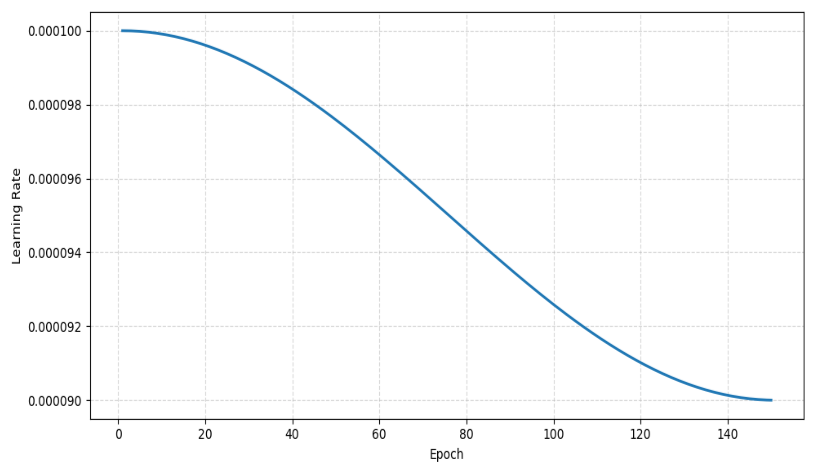
\includegraphics[width=0.5\textwidth]{img/cosine_annealing.png}
\caption{Decaimiento de la tasa de aprendizaje ($\eta$) bajo Cosine Annealing.}
\end{figure}

Esta política favorece la convergencia suave hacia mínimos más planos, reduciendo el riesgo de oscilaciones en etapas tardías del entrenamiento. 

También en algunos entrenamientos y a partir de épocas avanzadas se incorporó un criterio de descarte de muestras, en los que la cantidad de vóxeles NCR anotados era inferior a 500, de esta manera forzando al modelo a concentrarse en dicha clase una vez que la red ya había convergido sobre las más frecuentes.

\begin{figure}[H]
\centering
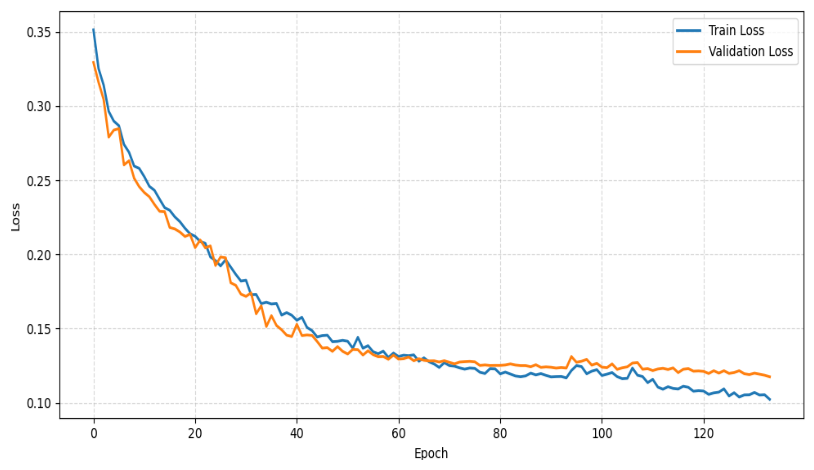
\includegraphics[width=0.5\textwidth]{img/best_annealing_3_losses.png}
\caption{Evolución de la función de pérdida en entrenamiento y validación (para el caso de \textit{Cosine annealing}).}
\end{figure}

La curva de validación acompaña consistentemente a la de entrenamiento sin evidenciar sobreajuste marcado, lo que sugiere que la regularización mediante \textit{Dropout3D} y el descarte de muestras con escasa anotación contribuyeron a una generalización adecuada. 

Los resultados concretos y comparaciones se abordan en la sección \nameref{sec:eval}.

\subsection{Limitaciones de Hardware}
\label{sec:limitaciones_hardware}

Como se mencionó anteriormente el entrenamiento de la U-Net 3D impone restricciones de memoria de video (VRAM) significativas, dado que un único \textit{forward pass} requiere cerca de $2GB$. Esto condicionó fuertemente el tamaño de mini-batch utilizable en cada entorno. 

Se dispuso de tres plataformas de cómputo con características distintas, resumidas en la siguiente tabla.

\begin{table}[H]
\centering
\label{tab:gpus}
\small
\setlength{\tabcolsep}{2pt} % default is 6pt
\begin{tabular}{|l|l|c|c|}
\hline
\textbf{Entorno} & \textbf{GPU} & \textbf{VRAM} & \textbf{Minibatch} \\
\hline
GPU local 1  & GTX 1050 Ti  & 4\,GB  & 1-2 \\
GPU local 2  & RTX 3070     & 8\,GB  & 2-4 \\
Colab (nube) & Tesla T4     & 16\,GB & 8 \\
\hline
\end{tabular}
\caption{Entornos de entrenamiento utilizados.}
\end{table}

La GPU local 1 (GTX 1050 Ti, 4\,GB VRAM) resultó insuficiente para mini-batches de tamaño 2, ya que incluso empleando \textit{mixed precision} con \textit{GradScaler}, se producían desbordamientos numéricos que impedían la convergencia, por lo que su uso quedó limitado a pruebas de integridad del pipeline.

La GPU local 2 (RTX 3070, 8\,GB VRAM), que fue cedida de forma temporal, permitió entrenar con mini-batches de hasta 4 muestras y constituyó el entorno principal para los experimentos más controlados. 

Finalmente, la Tesla T4 provista por Google Colab (16\,GB VRAM) admitió mini-batches de 8, acelerando la convergencia, aunque las restricciones de tiempo de sesión y cuota de uso limitaron la cantidad de experimentos ejecutables en esa plataforma.

\vspace{0.25cm}

En todos los entornos se utilizó \textit{prefetching} mediante \textit{workers} multi-processing (en CPU) para preparar los batches en RAM y transferirlos a VRAM de forma \textit{'lazy'}, reduciendo el tiempo de espera entre iteraciones. Este mecanismo también estuvo sujeto a restricciones (debido al tamaño del dataset), en entornos con poca RAM o pocos núcleos disponibles, y el cuello de botella se desplazó hacia la CPU durante la carga o ingesta y preprocesamiento de los volúmenes.

\section{Evaluación y Resultados}
\label{sec:eval}

A lo largo del proyecto se entrenaron y evaluaron más de 20 modelos, variando la política de tasa de aprendizaje, la ponderación de clases, el tamaño de mini-batch y la cantidad de épocas. De este proceso iterativo se consolidaron tres configuraciones con los mejores resultados en validación, cuyos detalles se presentan a continuación.

\begin{itemize}
    \item \textbf{Weighted Annealing}: Utiliza los pesos ajustados al imbalance de clases mencionados en la sección de \nameref{sec:loss_func} y \textit{Cosine annealing}.
    \item \textbf{Balanced Weights}: Utiliza $\eta$ constante y pesos equitativos.
    \item \textbf{Weighted}: Utiliza $\eta$ constante y pesos ajustados al imbalance de clases.
\end{itemize}


La evaluación se realizó sobre un conjunto de validación compuesto por 63 volúmenes (20\% del dataset total). Las métricas reportadas son el \textbf{Dice Score} y la \textbf{Intersección sobre Unión (IoU)}, calculadas por clase y promediadas, excluyendo el fondo en ambos casos.

Adicionalmente, cada inferencia incorpora \textbf{Test-Time Augmentation (TTA)}, para esto se promediaron las predicciones sobre la imagen original y tres versiones con volteo especular en cada eje espacial (D, H, W), obteniendo así estimaciones más robustas sin reentrenamiento adicional.

\subsection{Comparación de Modelos}

Los resultados para cada uno de los tres modelos mencionados se pueden apreciar en los siguientes cuadros:

\begin{table}[H]
\centering
\small
\setlength{\tabcolsep}{2pt}
\begin{tabular}{|l|c|c|c|}
\hline
\textbf{Modelo} & \textbf{NCR} & \textbf{ED} & \textbf{ET} \\
\hline
Weighted Annealing & 0.657 & 0.738 & 0.731 \\
Balanced Weights   & 0.672 & 0.763 & 0.761 \\
Weighted           & 0.654 & 0.754 & 0.756 \\
\hline
Ensamble (top 3)   & 0.669 & 0.759 & 0.755 \\
\hline
\end{tabular}
\caption{Dice Score por clase en validación.}
\label{tab:dice}
\end{table}

\begin{table}[H]
\centering
\small
\setlength{\tabcolsep}{2pt}
\begin{tabular}{|l|c|c|c|}
\hline
\textbf{Modelo} & \textbf{NCR} & \textbf{ED} & \textbf{ET} \\
\hline
Weighted Annealing & 0.529 & 0.614 & 0.609 \\
Balanced Weights   & 0.549 & 0.642 & 0.647 \\
Weighted           & 0.531 & 0.631 & 0.643 \\
\hline
Ensamble (top 3)   & 0.546 & 0.638 & 0.641 \\
\hline
\end{tabular}
\caption{IoU por clase en validación.}
\label{tab:iou_clase}
\end{table}

\begin{table}[H]
\centering
\small
\setlength{\tabcolsep}{2pt}
\begin{tabular}{|l|c|c|c|}
\hline
\textbf{Modelo} & \textbf{Épocas} & \textbf{$\text{Dice}$} & \textbf{$\text{IoU}$} \\
\hline
Weighted Annealing & 133 & 0.71 & 0.58 \\
Balanced Weights   & 168 & \textbf{0.73} & \textbf{0.61} \\
Weighted           & 99 & 0.72 & 0.60 \\
\hline
Ensamble (top 3)   & --- & 0.73 & 0.61 \\
\hline
\end{tabular}
\caption{Métricas medias en validación.}
\label{tab:medias}
\end{table}

Como se puede observar, por un lado la clase ED es consistentemente la mejor segmentada en todos los modelos, debido a su mayor volumen relativo y contraste marcado (en FLAIR), y por otro lado la clase NCR presenta consistentemente puntuaciones más bajas, probablemente debido a su morfología heterogénea y a sus límites poco definidos, lo que dificulta su discriminación en comparación con ED y ET.

El modelo \textbf{Balanced Weights} con 168 épocas obtuvo el mejor desempeño individual, alcanzando un Dice medio de \textbf{0.73} e IoU medio de \textbf{0.61}. 

El \textbf{ensamble} de los tres mejores modelos, que promedia las probabilidades predichas por cada uno antes de aplicar \textit{argmax}, igualó al mejor modelo individual en métricas medias (Dice 0.73, IoU 0.61) sin superarlo de forma apreciable. Esto sugiere que los tres modelos comparten sesgos similares producto de la misma arquitectura base, limitando la diversidad del ensamble.

\subsection{Ejemplos de Predicciones}

A continuación se visualizan algunas predicciones de volúmenes tomados al azar incluyendo los contrastes utilizados, la segmentación etiquetada real y la inferencia del mejor modelo. Se muestra en verde la región ED, en azul ET, y en rojo NCR.

\begin{figure}[H]
\centering
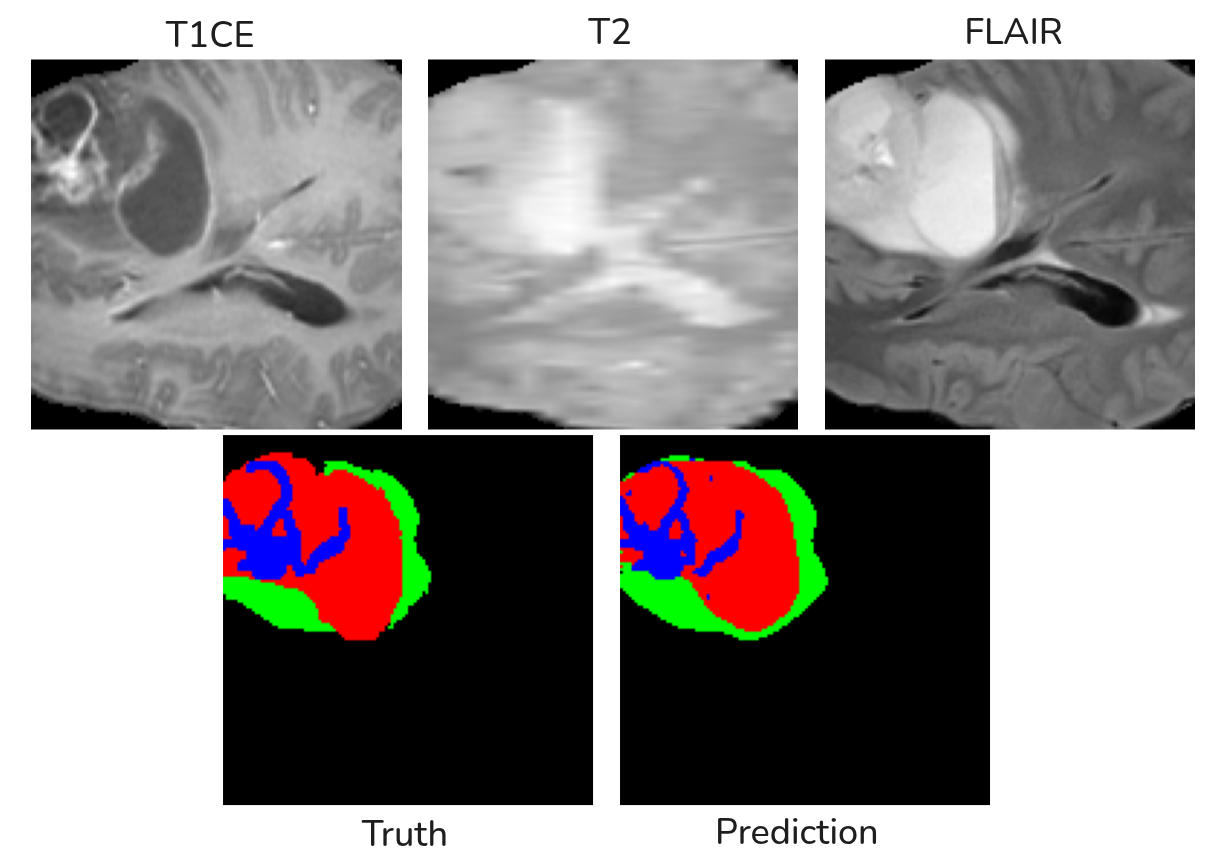
\includegraphics[width=0.5\textwidth]{img/264.png}
\caption{Inferencia segmentada sobre la muestra \#264.}
\end{figure}

\vspace{-2.5cm}
\begin{figure}[H]
\centering
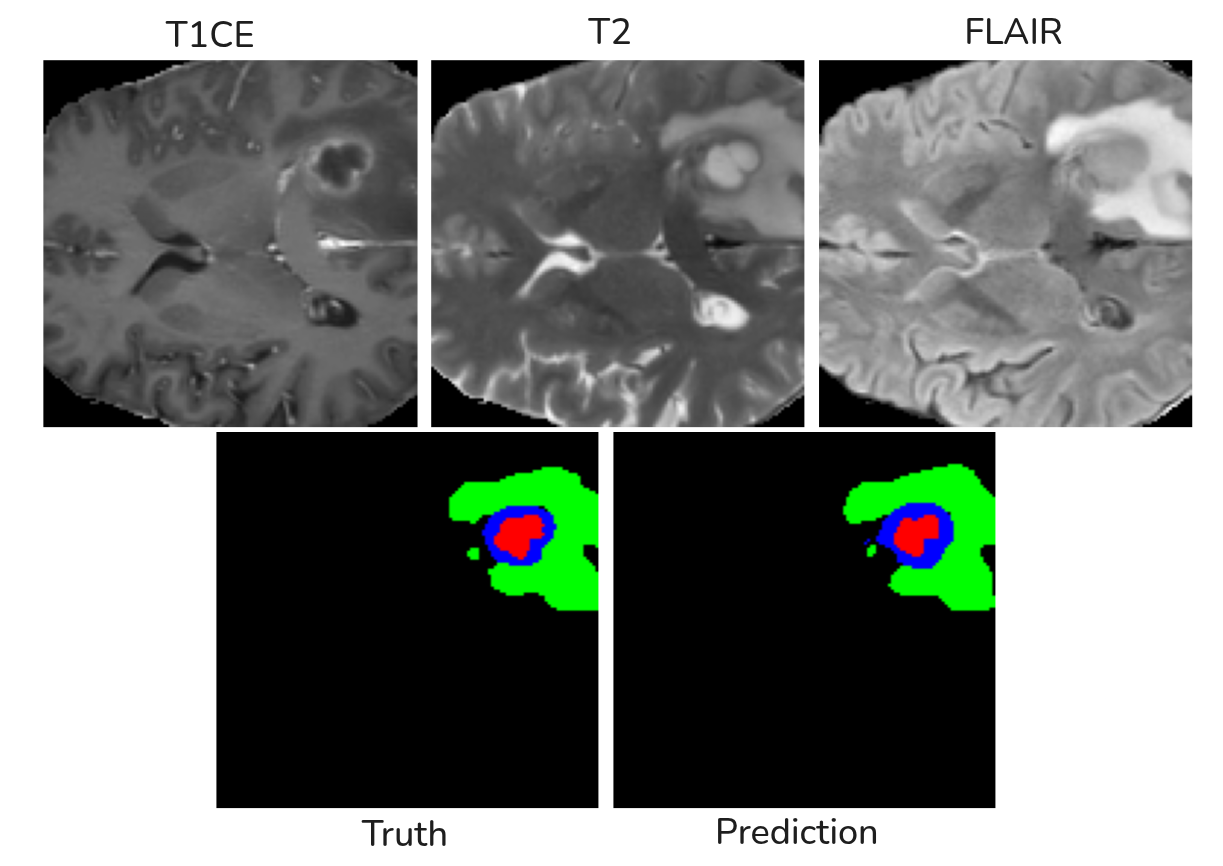
\includegraphics[width=0.5\textwidth]{img/337.png}
\caption{Inferencia segmentada sobre la muestra \#337.}
\end{figure}

\begin{figure}[H]
\centering
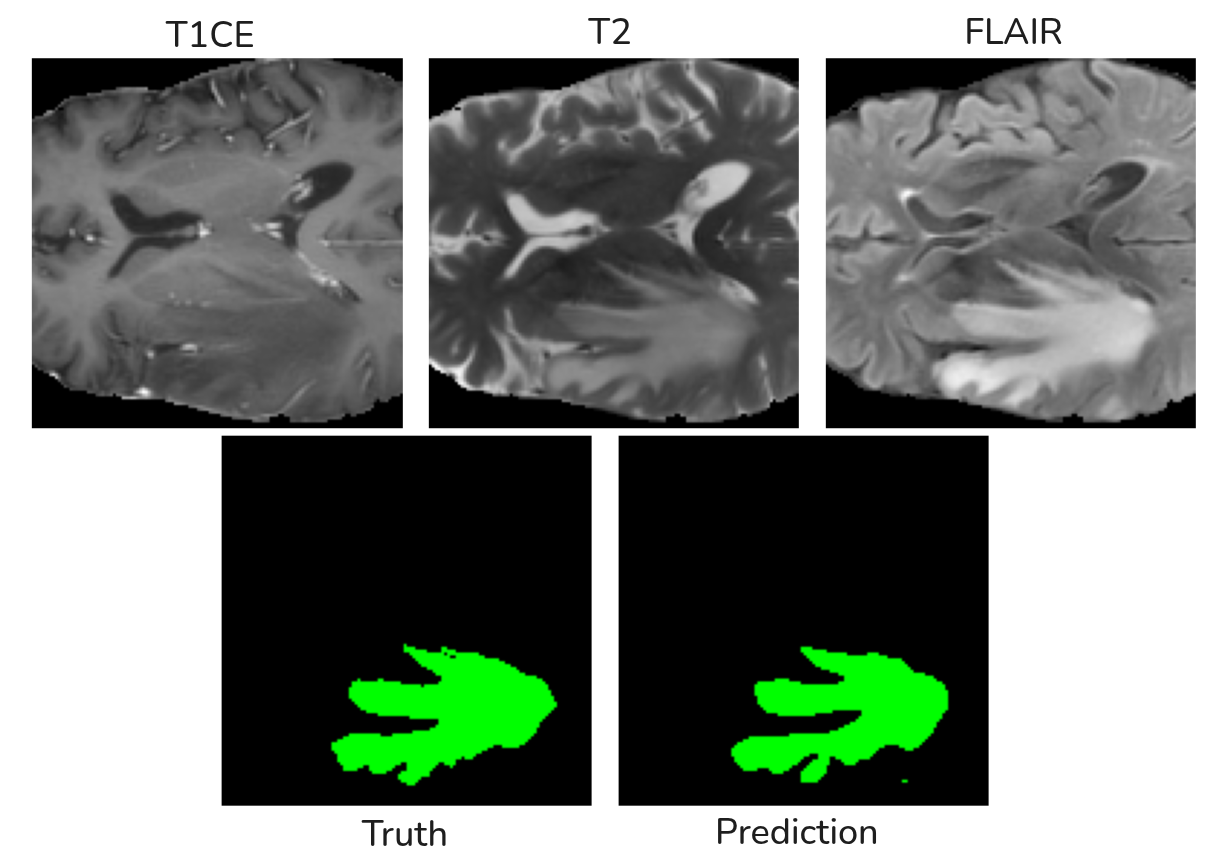
\includegraphics[width=0.5\textwidth]{img/351.png}
\caption{Inferencia segmentada sobre la muestra \#351 (solo ED).}
\end{figure}

Las predicciones visuales evidencian que el modelo captura correctamente la extensión general del tumor y delimita con razonable precisión las regiones, aunque con cierta variabilidad, correspondiéndose con lo que sugieren las métricas tomadas.

\section{Direcciones a Futuro}

Ademas de las posibles mejoras mencionadas a lo largo de las secciones y tomando el mejor modelo como base, a futuro el progreso se direcciona a la \textit{interpretabilidad}, en vistas de integrar algoritmos como \textit{Grad-CAM} en la arquitectura U-Net y generar reportes sobre la confianza e incertidumbre de las predicciones.
Esto asegurará que, en aplicaciones médicas, un experto podrá no solo emplear las inferencias en tiempo real, sino comprender y trazar eficientemente el margen de incerteza al tomar decisiones clínicas asociadas a patologías cerebrales.

\section{Conclusión}

En este trabajo se desarrolló un pipeline completo de segmentación semántica de tumores cerebrales en volúmenes 3D de resonancia magnética, desde el preprocesamiento del dataset BraTS 2020 hasta el entrenamiento y evaluación de múltiples configuraciones de una U-Net 3D, logrando un Dice Score medio de \textbf{0.73} e IoU medio de \textbf{0.61} en validación.

La exploración con modelos 2D livianos motivó la adopción de una arquitectura volumétrica, que demostró capturar correctamente el contexto espacial necesario para delimitar las regiones tumorales. Las principales limitaciones estuvieron asociadas al hardware disponible y al des-balance de clases, que afecta especialmente la segmentación de NCR. Como trabajo futuro se plantea incorporar explicabilidad y estimación de incertidumbre, orientados a mayor confiabilidad clínica.

\newpage
\clearpage

\begin{thebibliography}{99}

\bibitem{deeplearningmonograph}
Utrera, M. (2025--2026).
\textit{Brain Tumor Segmentation}.
GitHub repository.
\url{https://github.com/maxogod/Brain-Tumor-Segmentation}

\bibitem{hertz}
Hertz, J., Krogh, A., \& Palmer, R. G. (1991).
\textit{Introduction to the Theory of Neural Computation}.
Addison-Wesley.

% ---------------------------
% Understanding the field
% ---------------------------

\bibitem{brats2024}
Baid, U., et al. (2024).
The 2024 Brain Tumor Segmentation (BraTS) Challenge: Glioma Segmentation on Post-treatment MRI.
\url{https://arxiv.org/abs/2405.18368}

\bibitem{qubrats}
Jungo, A., et al. (2020).
QU-BraTS: MICCAI BraTS 2020 Challenge on Quantifying Uncertainty in Brain Tumor Segmentation -- Analysis of Ranking Scores and Benchmarking Results.
\textit{Frontiers in Neuroscience}, 14.
\url{https://www.researchgate.net/publication/369664632_QU-BraTS_MICCAI_BraTS_2020_Challenge_on_Quantifying_Uncertainty_in_Brain_Tumor_Segmentation_-_Analysis_of_Ranking_Scores_and_Benchmarking_Results}

% ---------------------------
% Understanding the models
% ---------------------------

\bibitem{unet}
Ronneberger, O., Fischer, P., \& Brox, T. (2015).
U-Net: Convolutional Networks for Biomedical Image Segmentation.
In \textit{Proceedings of MICCAI 2015} (pp. 234--241).
\url{https://arxiv.org/abs/1505.04597}

\bibitem{attentionunet}
Oktay, O., et al. (2018).
Attention U-Net: Learning Where to Look for the Pancreas.
\url{https://arxiv.org/abs/1804.03999}

\bibitem{mobilenetv2}
Sandler, M., Howard, A., Zhu, M., Zhmoginov, A., \& Chen, L.-C. (2018).
MobileNetV2: Inverted Residuals and Linear Bottlenecks.
In \textit{Proceedings of the IEEE Conference on Computer Vision and Pattern Recognition (CVPR)}.
\url{https://arxiv.org/abs/1801.04381}

\bibitem{gradcam}
Selvaraju, R. R., et al. (2017).
Grad-CAM: Visual Explanations from Deep Networks via Gradient-based Localization.
In \textit{Proceedings of the IEEE International Conference on Computer Vision (ICCV)}.
\url{https://arxiv.org/abs/1610.02391}

\bibitem{interpretability}
Tjoa, E., \& Guan, C. (2020).
A Survey on Explainable Artificial Intelligence (XAI): Toward Medical XAI.
\textit{IEEE Transactions on Neural Networks and Learning Systems}.
\url{https://arxiv.org/abs/1907.07374}

% ---------------------------
% Other solutions
% ---------------------------

\bibitem{autoencoderreg}
Myronenko, A. (2019).
3D MRI Brain Tumor Segmentation Using Autoencoder Regularization.
In \textit{Proceedings of MICCAI Brainlesion Workshop}.
\url{https://arxiv.org/abs/1810.11654}

\bibitem{crossattention}
Zhou, Z., Siddiquee, M. M. R., Tajbakhsh, N., \& Liang, J. (2020).
One-pass Multi-task Networks with Cross-task Guided Attention for Brain Tumor Segmentation.
\textit{IEEE Transactions on Medical Imaging}.
\url{https://arxiv.org/abs/1906.01796}

\bibitem{segformer3d}
Perera, M., et al. (2024).
SegFormer3D: An Efficient Transformer for 3D Medical Image Segmentation.
\url{https://arxiv.org/abs/2404.10156}
% TODO: Replace with the correct publication and URL.
% The identifier arXiv:2401.XXXX is incomplete.

% ---------------------------
% Transformers / Attention
% ---------------------------

\bibitem{transformers}
Vaswani, A., et al. (2017).
Attention Is All You Need.
In \textit{Advances in Neural Information Processing Systems (NeurIPS)}.
\url{https://arxiv.org/abs/1706.03762}

\end{thebibliography}
